\chapter{자발적 초대칭 깨짐과 첫 번째 \texorpdfstring{\(SU(5)\)}{SU(5)} 다중항}

\lectureoverview{대칭 깨짐은 먼저 스펙트럼에서 눈에 보이는 사실로 나타난다. 회전 대칭을 가진 원자에는 축퇴된 각운동량 준위가 있지만, 자기장을 걸면 이 준위들이 갈라진다. 강자성체는 방정식의 대칭성이 진공에서는 유지되지 않을 수도 있다는 더 미묘한 점을 보여 준다. 갭이 없는 마그논, 조건 \(J|0\rangle\neq0\), 그리고 영이 아닌 질서 매개변수는 같은 현상을 나타내는 세 가지 표현이다. 이 패턴을 카이랄 초대칭 장 이론으로 가져와 스칼라 퍼텐셜 \(V=|W'|^2\)을 유도하고, 보조장 \(F\)을 제거하여 초대칭이 보존되는 진공과 \(F\)항에 의해 초대칭이 깨지는 진공을 구별한다. 그에 따른 진공 에너지, 보손--페르미온 분리, 골드스티노, 숨은 부문, 초힉스 메커니즘을 살펴보며 초대칭 논의를 마무리한다. 마지막 부분에서는 주제를 바꾸어 대통일을 다룬다. \(SU(3)\times SU(2)\times U(1)\)은 \(SU(5)\)에 블록 단위로 포함되며, 첫 번째 물질 다중항은 렙톤 이중항과 아래형 반쿼크 세 개를 묶는다.}

\section{스펙트럼에 남는 대칭성의 흔적}

원자에서 시작하는 목적은 기초 양자역학을 복습하는 데 그치지 않는다. 에너지 준위와 입자 질량은 같은 종류의 스펙트럼 자료다. 대칭성이 원자 준위의 일치를 강제한다면, 대칭성이 깨질 때 그 준위가 갈라질 수 있다. 장 이론에서는 이에 대응해 입자 다중항의 구성원들이 서로 다른 질량을 얻을 수 있다.

원자 상태의 총각운동량을 \(j\)이라 하자. 여기에는 스핀과 궤도 각운동량이 모두 포함된다. 임의로 정한 축을 기준으로 하면
\begin{equation}
J_z|j,m\rangle=m\hbar|j,m\rangle,
\qquad
m=-j,-j+1,\ldots,j,
\end{equation}
따라서 상태는 \(2j+1\)개다. 교과서에서 익숙하게 보는 화살표를 각운동량 벡터가 공간에서 오직 \(2j+1\)개의 방향만 가질 수 있다는 뜻으로 받아들여서는 안 된다. 양자화되는 것은 선택한 축 방향의 성분이다.

비어 있는 회전 대칭 공간에서는 그 축을 특별히 택할 물리적 이유가 없다. 회전은 스핀 \(j\) 다중항 안에서 상태들을 서로 섞으며, 해밀토니안의 불변성은 다음을 뜻한다.
\begin{equation}
[H,\mathbf J]=0,
\qquad
E_{j,-j}=E_{j,-j+1}=\cdots=E_{j,j}.
\label{eq:l9-degeneracy}
\end{equation}

\begin{classroomqa}
\audiencequestion{원자 전체를 회전해도 에너지가 변하지 않는다는 것을 보장하는 대칭성은 무엇인가요? \lecturetimestamp{00:05:53}}
\lecturerresponse{회전 대칭성입니다. 회전은 물리계를 바꾸지 않은 채 각운동량의 한 방향을 다른 방향으로 바꾸므로, \(2j+1\)개의 상태는 모두 에너지가 같습니다.}
\end{classroomqa}

이제 자기장 \(\mathbf B=B\hat{\mathbf z}\)을 걸어 보자. 상호작용은
\begin{equation}
H_B=-\boldsymbol{\mu}\cdot\mathbf B
\end{equation}
자기장과 나란한 성분을 구별한다. 개략적으로는 다음과 같다.
\begin{equation}
\Delta E_m\propto mB.
\label{eq:l9-zeeman}
\end{equation}
약한 자기장에서는 \(m\)가 서로 다른 준위들이 선형적으로 갈라지고, 이들 사이의 전이로 스펙트럼 선도 분리된다.

\begin{classroomqa}
\audiencequestion{자기장에 의한 원자 준위의 분리를 무엇이라 하나요? \lecturetimestamp{00:07:13}}
\lecturerresponse{제만 효과입니다. 이것이 전체 논의의 원형입니다. 대칭성이 축퇴시킨 준위는 배경장이 그 대칭성을 깨면 갈라집니다.}
\end{classroomqa}

\begin{center}
\begin{tikzpicture}[x=1.05cm,y=0.75cm,>=Latex]
  \draw[thick] (-3,0) -- (-1,0);
  \node[left] at (-3,0) {\(B=0\)};
  \foreach \y/\m in {-1.2/-1,-0.4/0,0.4/1,1.2/2} {
    \draw[thick,teal!70!black] (1,\y) -- (3,\y);
    \node[right] at (3,\y) {\(m=\m\)};
  }
  \draw[->,thick] (-0.5,0) -- (0.6,0);
  \node[above] at (0.05,0) {\(\mathbf B\neq0\)};
\end{tikzpicture}
\end{center}

\section{강자성체: 대칭적인 법칙과 비대칭적인 진공}

강자성체를 설명하는 간단한 미시적 그림에서는 각 격자점에 작은 자기 모멘트가 있다고 본다. 이웃한 모멘트들이 평행하게 정렬될 때 에너지가 낮아진다면 저온 상은 강자성체가 된다. 반평행 정렬이 선호되면 반강자성체가 된다. 강한 열 요동이나 양자 요동이 있으면 순자화가 사라질 수도 있다.

강자성체가 우주 전체를 채우고 모멘트가 한 방향으로 고르게 정렬된 상태에 놓여 있다고 하자. 내부 자기장은 외부에서 가한 자기장과 마찬가지로 원자 준위를 분리한다. 하지만 결정적인 차이가 있다. 근본 상호작용은 북쪽이나 동쪽 또는 다른 어떤 방향도 선호하지 않는다. 방향을 고르게 회전시킨 모든 배치는 같은 에너지를 갖는다.
\begin{equation}
\mathbf M(\mathbf x)=M_0\hat{\mathbf n},
\qquad
\hat{\mathbf n}\in S^2.
\label{eq:l9-ferromagnetic-vacua}
\end{equation}
방정식은 회전 대칭이지만, 실제 바닥 상태 하나는 \(\hat{\mathbf n}\)를 택한다. 이것은 명시적 대칭 깨짐이 아니라 자발적 대칭 깨짐이다.

이 매질의 들뜸으로 이루어진 거주자는 우주 전체를 붙잡아 회전시킬 수 없다. 따라서 국소적으로 보면 선택된 방향은 외부 자기장의 방향만큼이나 근본적인 것처럼 보인다. 원자는 여전히 같은 준위 패턴을 보지만, 각운동량은 외부에서 정한 \(z\)축이 아니라 \(\hat{\mathbf n}\)을 기준으로 분해된다. 내부 관찰자가 겉보기의 비대칭성이 법칙이 아니라 상태에 속한다는 것을 어떻게 알아낼 수 있을까?

\subsection{골드스톤 판별법}

모든 모멘트의 방향을 고르게 회전시키면 ~\eqref{eq:l9-ferromagnetic-vacua}의 한 진공에서 다른 진공으로 옮겨가며, 에너지는 들지 않는다. 이제 방향이 공간에서 매우 천천히 변하도록 하자. 이웃한 모멘트들이 서로 당기면서 변형이 스핀파로 전파되고, 그 양자가 마그논이다. 파장이 무한대로 커지면 배치는 균일한 회전에 가까워지므로 들뜸 에너지는 0으로 간다.
\begin{equation}
k=\frac{2\pi}{\lambda}\longrightarrow0
\quad\Longrightarrow\quad
E(k)\longrightarrow0.
\label{eq:l9-gapless-magnon}
\end{equation}
두 관찰자는 가까운 모멘트들을 흔들어 이런 파동을 매질에 전달하고, 임의로 낮은 에너지를 측정할 수 있다. 우주를 회전시킬 수 없어도 이 실험으로 자발적 대칭 깨짐을 알아낼 수 있다.

\editorialnote{강자성 마그논은 갭이 없지만, 일반적으로 상대론적 분산 관계 \(E\propto|k|\)가 아니라 비상대론적 이차 분산 관계 \(E\propto k^2\)를 따른다. 이 강의에서 무질량이라는 말은 물리적으로 중요한 의미, 즉 갭이 사라진다는 뜻으로 쓰인다. 두 경우 모두 골드스톤 모드다.}

같은 발상은 입자물리학의 게이지 군과 맛깔 군을 비롯한 연속 내부 대칭에도 적용된다. 다만 깨진 대칭이 게이지 대칭이면 골드스톤 모드는 독립적인 무질량 입자로 남지 않는다.

\begin{classroomqa}
\audiencequestion{자발적 대칭 깨짐이 게이지 불변성과 함께 나타나면 어떻게 되나요? \lecturetimestamp{00:15:56}}
\lecturerresponse{골드스톤 보손은 게이지장의 편극을 하나 더 제공하고, 게이지 보손은 질량을 얻습니다. 이것이 힉스 메커니즘이며, 중력과의 유사성을 다룰 때 다시 살펴보겠습니다.}
\end{classroomqa}

\section{대칭 깨짐을 나타내는 서로 동등한 세 가지 신호}

이제 강자성체를 서로 보완하는 세 가지 언어로 기술할 수 있다.

\paragraph{축퇴된 진공.}
방향 \(\hat{\mathbf n}\)마다 에너지가 최소인 상태가 하나씩 있다. 대칭성은 이 상태들을 서로 연결하지만, 물리계는 이 계열 가운데 하나를 택해 그 안에서 일어난다.

\paragraph{진공을 소멸시키지 않는 생성자.}
\(J_a\)를 회전 생성자라 하자. 유한한 변환은
\begin{equation}
U(\epsilon)=e^{-i\epsilon J_a},
\end{equation}
이며, \(J_a|0\rangle\)은 회전된 상태 전체가 아니라 진공의 무한소 변화에 비례한다.

\begin{classroomqa}
\audiencequestion{회전 대칭의 생성자는 무엇인가요? \lecturetimestamp{00:17:29}}
\lecturerresponse{총각운동량의 성분입니다. 이를 \(J_a\)라고 부르는 까닭은 원자 하나만이 아니라 상태 전체를 회전시키기 때문입니다.}
\end{classroomqa}

깨지지 않은 생성자는 다음을 만족한다.
\begin{equation}
J_a|0\rangle=0.
\label{eq:l9-unbroken-generator}
\end{equation}
반면 깨진 생성자는 다음을 준다.
\begin{equation}
J_a|0\rangle\neq0.
\label{eq:l9-broken-generator}
\end{equation}

\begin{classroomqa}
\audiencequestion{\(J_a|0\rangle\)가 영이 아니면 단순히 같은 진공을 주나요? \lecturetimestamp{00:19:43}}
\lecturerresponse{아닙니다. 선택된 진공과 그것을 아주 조금 회전시킨 진공 사이의 무한소 차이를 줍니다. 물리적으로 이 차이는 파장이 무한히 긴 골드스톤 들뜸입니다.}
\end{classroomqa}

\begin{classroomqa}
\audiencequestion{이 무한소 회전으로 에너지가 바뀌나요? \lecturetimestamp{00:20:14}}
\lecturerresponse{아닙니다. 회전한 진공은 원래 진공과 축퇴되어 있으므로, 운동량이 0인 골드스톤 상태의 에너지도 0입니다.}
\end{classroomqa}

기호로 쓰면 다음과 같다.
\begin{equation}
J_a|0\rangle
\sim
|\pi_a,\mathbf k=0\rangle,
\label{eq:l9-generator-goldstone}
\end{equation}
여기서 \(\pi_a\)는 깨진 생성자에 대응하는 골드스톤 모드를 뜻한다.

\paragraph{영이 아닌 질서 매개변수.}
국소 자화 \(\mathbf M(\mathbf x)\)는 장이다. 고온상이거나 양자적으로 무질서한 상에서는
\begin{equation}
\langle\mathbf M\rangle=0,
\end{equation}
진공이 특정 방향을 선택하지 않는다. 질서가 있는 상에서는
\begin{equation}
\langle M_i\rangle\neq0
\quad\text{for at least one component }i,
\label{eq:l9-magnetization-order}
\end{equation}
회전하면 그 영이 아닌 성분이 다른 성분들과 섞인다. 축퇴된 진공, 깨진 생성자, 영이 아닌 질서 매개변수라는 세 가지 패턴을 초대칭 논의에 적용한다.

\section{키랄 다중항 복습}

가장 단순한 4차원 예에는 복소 스칼라 하나, 바일 페르미온 하나, 보조 복소 스칼라 하나가 들어 있다. 키랄 좌표는
\begin{equation}
y^\mu=x^\mu+i\bar\theta\bar\sigma^\mu\theta,
\end{equation}
이며, 키랄 초장은 개략적으로 다음과 같이 전개된다.
\begin{equation}
\Phi(y,\theta)=
\phi(y)+\sqrt2\,\theta\psi(y)+\theta^2F(y).
\label{eq:l9-chiral-expansion}
\end{equation}
이 강의에서는 관례적인 계수 \(\sqrt2\)를 생략했지만, 이제부터는 성분의 계수를 표준형으로 맞추기 위해 이를 포함한다. 키랄 초장은 본질적으로 복소수다. 실수 조건을 부과해도 초대칭 변환 아래에서 그 조건은 보존되지 않는다.

초대칭 운동 작용은
\begin{equation}
S_{\mathrm{kin}}
=
\int d^4x\,d^4\theta\,
\Phi^\dagger\Phi.
\label{eq:l9-kahler-action}
\end{equation}
으로 주어진다. 그라스만 적분은 \(\theta^2\bar\theta^2\)의 계수를 선택한다. 계량 부호 규약을 대부분 음수로 잡으면 성분 표현은 다음과 같다.
\begin{equation}
\mathcal L_{\mathrm{kin}}
=
\partial_\mu\phi^\ast\,\partial^\mu\phi
+i\bar\psi\bar\sigma^\mu\partial_\mu\psi
+F^\ast F.
\label{eq:l9-chiral-kinetic}
\end{equation}
앞의 두 항은 스칼라와 페르미온을 전파시킨다. 마지막 항에는 미분이 없으므로 입자를 전파시키지 않는다.

\begin{figure}[H]\centering
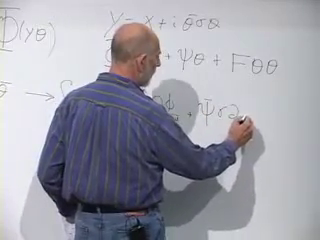
\includegraphics[width=0.76\textwidth]{lecture_09_figure_02.png}\lectureframe{00:27:36.000}\caption{스칼라, 페르미온, 보조장 항 위에 표시한 키랄 좌표와 성분 전개.}\end{figure}

\section{적분이 선택하는 것: \texorpdfstring{\(d^2\theta\)}{2} 적분}

상호작용과 질량은 초퍼텐셜인 정칙 함수 \(W(\Phi)\)에서 나온다.
\begin{equation}
S_W
=
\int d^4x
\left[
\int d^2\theta\,W(\Phi)
+\mathrm{h.c.}
\right].
\label{eq:l9-superpotential-action}
\end{equation}
키랄 표현에는 독립적인 \(\bar\theta\) 의존성이 없으므로 네 개의 반대칭 좌표 모두에 대해 적분하면 0이 된다. 대신 \(d^2\theta\) 적분은 그 표현의 \(\theta^2\) 성분을 선택한다.

일반 함수를 다루기 전에 계수 조합을 살펴보기 위해 \(W(\Phi)=\Phi^n\)라 하자. 다음 식에서
\begin{equation}
(\phi+\sqrt2\,\theta\psi+\theta^2F)^n,
\end{equation}
정확히 두 개의 \(\theta\)를 얻는 방법은 두 가지다. \(F\theta^2\) 하나를 택하거나 페르미온 인자를 두 개 택할 수 있다.

\begin{classroomqa}
\audiencequestion{하나의 \(F\theta^2\)를 택하고 나머지는 스칼라인 항은 몇 개 있나요? 스칼라는 \(n-1\)개 또는 \(n\)개인가요? \lecturetimestamp{00:31:33}}
\lecturerresponse{\(n\)개입니다. \(n\)개의 인자 가운데 어느 하나에서 \(F\theta^2\)를 택할 수 있고, 나머지 \(n-1\)개 인자는 \(\phi\)를 제공합니다. 따라서 기여항은 \(nF\phi^{n-1}\)입니다.}
\end{classroomqa}

\begin{classroomqa}
\audiencequestion{두 인자에서 페르미온 두 개를 얻는 방법은 몇 가지인가요? \lecturetimestamp{00:32:26}}
\lecturerresponse{순서 없는 선택은 \(\binom n2=n(n-1)/2\)가지입니다. 그라스만 수축이 이에 해당하는 \(\psi\psi\) 항을 정합니다.}
\end{classroomqa}

따라서 강의에서 계수를 생략한 표기법으로는 다음과 같다.
\begin{equation}
\int d^2\theta\,\Phi^n+\mathrm{h.c.}
\;\leadsto\;
nF\phi^{n-1}
-\frac{n(n-1)}{2}\phi^{n-2}\psi\psi
+\mathrm{h.c.}
\label{eq:l9-power-extraction}
\end{equation}
여기서 보인 마이너스 부호는 표준 정규화 전개와 그라스만 규약에서 나온다. 규약을 바꾸면 겉으로 드러나는 부호가 달라질 수 있다.

\begin{classroomqa}
\audiencequestion{\(\phi^n\)처럼 \(\theta\)가 하나도 없는 항은 어떻게 되었나요? \lecturetimestamp{00:33:10}}
\lecturerresponse{곱에는 들어 있지만 \(d^2\theta\)가 이를 버립니다. 화살표는 적분이 \(\theta^2\) 계수를 선택한다는 뜻이지, 전체 표현들이 같다는 뜻은 아닙니다.}
\end{classroomqa}

\begin{figure}[H]\centering
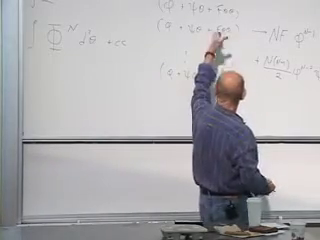
\includegraphics[width=0.82\textwidth]{lecture_09_figure_03.png}\lectureframe{00:33:38.000}\caption{반복되는 초장 인자들과, 두 \(\theta\) 성분을 등호가 아니라 추출한다는 뜻을 나타내는 함의 화살표.}\end{figure}

임의의 계수를 갖는 거듭제곱들을 모두 더하면 조합 계수가 도함수로 바뀐다.
\begin{equation}
\int d^2\theta\,W(\Phi)+\mathrm{h.c.}
\;\leadsto\;
F W'(\phi)
-\frac12 W''(\phi)\psi\psi
+\mathrm{h.c.}
\label{eq:l9-W-components}
\end{equation}

\begin{classroomqa}
\audiencequestion{\(\phi^{n-2}\) 대신 \(\phi^{n-1}\)가 페르미온 항에 들어가는 이유는 무엇인가요? \lecturetimestamp{00:36:32}}
\lecturerresponse{두 인자에서 이미 페르미온을 얻었으므로 스칼라 인자는 \(n-2\)개 남습니다. 계수는 2계 도함수 \(W''(\phi)\)의 절반입니다.}
\end{classroomqa}

페르미온 항은 중요하다. \(W''\)가 상수이면 질량을 주고, \(W''\)가 \(\phi\)에 의존하면 유카와 상호작용을 준다. 하지만 진공을 분석할 때는 보조장 항 \(FW'\)가 즉각적인 정보를 담고 있다.

\section{보조장 제거}

\(F\)을 포함하는 항들을 모으면 다음과 같다.
\begin{equation}
\mathcal L_F
=
F^\ast F
+F W'(\phi)
+F^\ast \overline{W'(\phi)}.
\label{eq:l9-LF}
\end{equation}
\(\partial_\mu F\)가 없으므로 완전한 오일러--라그랑주 방정식
\begin{equation}
\partial_\mu
\frac{\partial\mathcal L}{\partial(\partial_\mu F)}
-
\frac{\partial\mathcal L}{\partial F}
=0
\end{equation}
은 곧바로 대수 방정식으로 단순화된다. \(F\)와 \(F^\ast\)를 독립 변수로 취급하면
\begin{align}
\frac{\partial\mathcal L_F}{\partial F}
&=F^\ast+W'(\phi)=0,
&
\frac{\partial\mathcal L_F}{\partial F^\ast}
&=F+\overline{W'(\phi)}=0,
\label{eq:l9-F-eom}
\end{align}
를 얻고, 따라서
\begin{equation}
F^\ast=-W'(\phi),
\qquad
F=-\overline{W'(\phi)}.
\label{eq:l9-F-solution}
\end{equation}

\begin{figure}[H]\centering
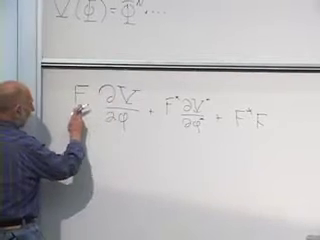
\includegraphics[width=0.82\textwidth]{lecture_09_figure_04.png}\lectureframe{00:39:40.000}\caption{가림 요소를 치운 뒤 보드에 함께 드러난 보조장 항 전체와 그 운동 방정식.}\end{figure}

\begin{classroomqa}
\audiencequestion{보드에 적힌 켤레장의 도함수가 아니라 \(\phi\)에 대해 미분해야 하지 않나요? \lecturetimestamp{00:41:21}}
\lecturerresponse{그렇습니다. 수정하면 ~\eqref{eq:l9-F-eom}에서 켤레 관계를 복원합니다. 즉 \(F^\ast=-W'(\phi)\)와 \(F=-\overline{W'(\phi)}\)입니다.}
\end{classroomqa}

~\eqref{eq:l9-LF}에 대입하면 다음을 얻는다.
\begin{equation}
\mathcal L_F\big|_{\mathrm{on\ shell}}
=-|W'(\phi)|^2.
\end{equation}
스칼라 라그랑지안은 운동 에너지에서 퍼텐셜 에너지를 뺀 형태이므로, 통상적인 스칼라 퍼텐셜은
\begin{equation}
\boxed{V(\phi,\phi^\ast)=|W'(\phi)|^2\ge0.}
\label{eq:l9-F-potential}
\end{equation}
이 \(V\)는 초퍼텐셜이 아니다. 정칙 초공간 함수에는 \(W\)를, 통상적인 퍼텐셜 에너지에는 \(V\)를 쓰겠다.

\subsection{바로 얻는 두 가지 예}

표준 규약에 따른 정규화를 사용하면
\begin{equation}
\begin{gathered}
W(\Phi)=\frac12m\Phi^2,\\
W'(\phi)=m\phi,
\qquad V=|m|^2|\phi|^2.
\end{gathered}
\label{eq:l9-quadratic-W}
\end{equation}
같은 항이 페르미온 질량 \(-\tfrac12m\psi\psi+\mathrm{h.c.}\)도 주므로, 초대칭이 깨지기 전에는 스칼라와 페르미온의 질량이 같다.

\begin{equation}
W(\Phi)=\frac{g}{3}\Phi^3,
\end{equation}을 가정하면
\begin{equation}
\begin{gathered}
W'(\phi)=g\phi^2,
\qquad V=|g|^2|\phi|^4,\\
\mathcal L_{\mathrm{Yukawa}}
=-g\phi\psi\psi+\mathrm{h.c.}
\end{gathered}
\label{eq:l9-cubic-W}
\end{equation}
사차 스칼라 꼭짓점은 두 스칼라의 산란을 나타내고, 유카와 항은 이에 대응하는 초대칭 짝이다.

\section{두 종류의 진공}

진공은 \(V\)가 최소인 상수 장 배치이며, 그 미분항은 사라진다. 식~\eqref{eq:l9-F-potential}이 음이 아니므로 가능한 경우는 두 가지다.

\subsection{에너지가 0인 최소점}

어떤 \(\phi_0\)가 다음을 만족하면
\begin{equation}
W'(\phi_0)=0,
\end{equation}
그러면
\begin{equation}
V(\phi_0)=0,
\qquad
\langle F\rangle=0.
\label{eq:l9-unbroken-F}
\end{equation}
진공은 초대칭을 보존한다. 이는 자화가 영인 경우에 해당한다. 어떤 보조장 성분도 초공간의 방향을 선택하지 않은 것이다.

\subsection{높아진 최소점}

최소점에서 방정식들
\begin{equation}
W'(\phi)=0
\label{eq:l9-F-flatness}
\end{equation}
을 동시에 만족하는 해가 없다면
\begin{equation}
V_{\min}>0,
\qquad
\langle F\rangle\neq0,
\label{eq:l9-broken-F}
\end{equation}
초대칭은 자발적으로 깨진다. 작용은 여전히 초대칭이지만, 가장 낮은 에너지 상태는 그렇지 않다.

\begin{figure}[H]\centering
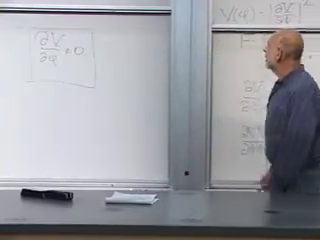
\includegraphics[width=0.88\textwidth]{lecture_09_figure_05.png}\lectureframe{00:52:09.960}\caption{양의 퍼텐셜, \(F\) 방정식, 진공 조건을 보드에 함께 제시하면서 대칭적인 방정식과 대칭을 따르지 않는 해를 구별한다.}\end{figure}

페르미온 변환을 통해 질서 매개변수에 관한 진술을 엄밀하게 표현할 수 있다.
\begin{equation}
\delta\psi_\alpha
=
i\sqrt2
(\sigma^\mu\bar\epsilon)_\alpha\partial_\mu\phi
+\sqrt2\,\epsilon_\alpha F.
\label{eq:l9-fermion-transformation}
\end{equation}
균일한 진공에서는 미분항이 사라진다. \(\langle F\rangle\neq0\)이면 초대칭 변환이 페르미온을 영이 아닌 상수만큼 이동시키므로 진공은 불변일 수 없다.\editorialnote{~\eqref{eq:l9-fermion-transformation}은 초장 성분들이 서로 변환된다는 강의의 설명을 명시적으로 보여 주는 표준 성분 형식이다.}

초대칭 대수에서도 같은 결론을 얻는다. 정지계에서는
\begin{equation}
\{Q_\alpha,Q_{\dot\alpha}^\dagger\}
=2\sigma^0_{\alpha\dot\alpha}H.
\end{equation}
진공 기대값을 취하면 에너지는 진공에 작용하는 초전하들의 노름의 합으로 표현된다.
\begin{equation}
E_0\ge0,
\qquad
E_0=0
\ \Longleftrightarrow\
Q_\alpha|0\rangle
=Q_{\dot\alpha}^\dagger|0\rangle=0.
\label{eq:l9-algebra-vacuum-energy}
\end{equation}
따라서 양의 진공 에너지와 자발적 초대칭 깨짐은 강체 초대칭에서 같은 진술의 두 측면이다.

\begin{center}
\begin{tikzpicture}[x=1.2cm,y=1.0cm,>=Latex]
  \draw[->] (-3,0) -- (-0.2,0) node[right] {\(\phi\)};
  \draw[->] (-2.8,-0.15) -- (-2.8,2.1) node[above] {\(V\)};
  \draw[thick,teal!75!black,domain=-2.5:-0.5,samples=60]
    plot (\x,{0.65*(\x+1.5)^2});
  \fill (-1.5,0) circle (2pt);
  \node[below] at (-1.5,0) {\(F=0\)};
  \draw[->] (0.4,0) -- (3.2,0) node[right] {\(\phi\)};
  \draw[->] (0.6,-0.15) -- (0.6,2.1) node[above] {\(V\)};
  \draw[thick,orange!85!black,domain=0.9:2.9,samples=60]
    plot (\x,{0.55*(\x-1.9)^2+0.65});
  \fill (1.9,0.65) circle (2pt);
  \draw[dashed] (0.6,0.65) -- (1.9,0.65);
  \node[below] at (1.9,0.65) {\(F\neq0\)};
\end{tikzpicture}
\end{center}

\editorialnote{간단한 예로 \(W=f\Phi\)를 들 수 있다. 이 경우 \(W'=f\)는 결코 사라지지 않으며 \(V=|f|^2\)이다. 이 한 장 모형에는 평탄한 스칼라 방향이 있다. 안정적인 \(F\)항 깨짐을 현실적으로 구현할 때는 보통 여러 카이랄 장을 사용하며, 오라페르타이형 숨은 부문이 그 예다.}

\section{초대칭 깨짐이 낳는 것}

\subsection{질량 분리}

이제 강자성체의 비유는 다시 스펙트럼에 관한 이야기로 이어진다. 약한 내부 자기장은 원자의 동일성을 없애지 않으면서 원자 준위를 분리한다. 마찬가지로 약하게 전달된 초대칭 깨짐 질서 매개변수는 그렇지 않았다면 한 초다중항에 속했을 보손과 페르미온을 분리한다.

\begin{classroomqa}
\audiencequestion{초대칭이 서로 변환시키며, 진공이 깨질 때 질량 축퇴를 잃는 입자는 무엇인가요? \lecturetimestamp{00:51:40}}
\lecturerresponse{보손과 페르미온입니다. 이들을 서로 연결하는 변환을 상태가 더 이상 따르지 않으면 질량이 같을 필요가 없습니다.}
\end{classroomqa}

분리는 \(\langle F\rangle\)만으로 생기는 것이 아니다. 깨짐을 가시 부문 장에 전달하는 결합에 달려 있다. 결합이 약하면 가시 입자들은 여전히 식별 가능하며, 질량 분리는 대통일 척도나 플랑크 척도보다 훨씬 작다. 결합이 강하다면, 엄청난 자기장 때문에 원자가 길게 늘어나 알아볼 수 없게 되는 상황에 비유할 수 있다.

\subsection{골드스티노}

일반적인 깨진 생성자에서는 \(J|0\rangle\)가 보손 골드스톤 상태를 준다. 초전하는 페르미온 생성자이며 보손 상태를 페르미온 상태로 바꾼다. 진공은 보손 상태로 간주되므로, 깨진 초전하는 에너지가 0인 페르미온 상태를 만든다.
\begin{equation}
Q_\alpha|0\rangle
\sim
|\widetilde G_\alpha,\mathbf k=0\rangle.
\label{eq:l9-goldstino}
\end{equation}
이 상태가 전파되는 형태는 무질량 바일 페르미온이며, 골드스톤 페르미온 또는 골드스티노라 부른다.

\begin{classroomqa}
\audiencequestion{초대칭 변환이 진공을 그대로 두지 않는다면 어떤 새로운 상태를 만들까요? \lecturetimestamp{00:53:24}}
\lecturerresponse{무질량 페르미온입니다. 일반적인 골드스톤 정리의 구조는 그대로지만, 페르미온 생성자가 보손 진공을 골드스티노로 바꿉니다.}
\end{classroomqa}

따라서 강체 초대칭의 자발적 깨짐에는 다음 두 가지 징후가 반드시 따른다.
\begin{equation}
\boxed{
V_{\min}>0
\qquad\text{and}\qquad
\text{a massless goldstino}.
}
\label{eq:l9-rigid-breaking-signatures}
\end{equation}

\section{숨은 부문}

원자와 강자성체를 두 부문으로 볼 수 있다. 강자성체에서는 질서 매개변수가 생기고, 원자는 거기서 전달된 장만 느낀다. 결합이 약하면 원자를 조작해도 마그논은 거의 들뜨지 않으므로 자기 매질에 직접 접근하기 어렵다. 이때 강자성체는 숨은 부문이지만, 작은 스펙트럼 분리를 통해 그 존재를 추론할 수 있다.

초대칭 모형 구축에서도 같은 용어를 사용한다. 숨은 부문의 추가 장들이 영이 아닌 \(F\)항 또는 \(D\)항 기댓값을 갖는다. 매개 메커니즘이라 불리는 상호작용은 그 깨짐을 가시 부문에 전달해 초대칭 짝들의 연성 질량을 만든다. 약한 전달은 훨씬 높은 근본 에너지 척도에서도 가시 이론이 근사적으로 초대칭을 유지하면서, 낮은 에너지에서는 보손--페르미온 사이에 정확한 축퇴가 나타나지 않을 수 있음을 설명해 준다.

이런 구성이 저절로 되는 것은 아니다. 추가 장, 안정적인 깨짐 진공, 제어 가능한 매개 메커니즘이 필요하다. 그래서 강의에서는 현실적인 초대칭 깨짐을 최소 모형에서 필연적으로 따라 나오는 단일 결과가 아니라 복잡하고 다소 인위적인 구성이라고 설명한다.

\section{중력은 두 가지 징후를 모두 바꾼다}

\subsection{진공 에너지가 중력의 원천이 된다}

중력이 없으면 모든 에너지에 상수를 더해도 비중력 실험은 달라지지 않는다. 중력이 있으면 진공 에너지 밀도는 우주상수로 아인슈타인 방정식에 들어간다. 양의 \(V_{\min}\)는 가속 팽창을 일으킨다. 그 척도가 초대칭 짝의 질량에 필요한 입자물리학 척도에 가깝다면, 그에 따른 곡률은 관측된 값보다 엄청나게 커진다.

\begin{classroomqa}
\audiencequestion{중력을 포함하면 양의 영이 아닌 진공 에너지는 우주에 어떤 영향을 미치나요? \lecturetimestamp{01:00:40}}
\lecturerresponse{우주상수로 작용해 가속 팽창을 일으킵니다. 보통의 입자물리학 에너지 척도에서는 그 효과가 도저히 감당할 수 없을 만큼 큽니다.}
\end{classroomqa}

국소 초대칭, 즉 초중력은 양의 제곱합 공식을 바꾼다. 참고로 표준 \(N=1\) \(F\)항 퍼텐셜은 다음과 같다.
\begin{equation}
\begin{aligned}
V_F={}&e^{K/M_P^2}
\left(
K^{i\bar j}D_iW\,D_{\bar j}\overline W
-\frac{3|W|^2}{M_P^2}
\right),\\
D_iW={}&\partial_iW+\frac{\partial_iK}{M_P^2}W.
\end{aligned}
\label{eq:l9-sugra-potential}
\end{equation}
음의 항이 있으므로 초대칭 깨짐에서 나온 양의 에너지는 원리상 일부 상쇄될 수 있다. 나머지는 작은 우주상수일 수 있다.

\editorialnote{강의에서는 의도적으로 개략적인 보정항만 제시하며 플랑크 질량의 위치에도 의문을 제기한다. ~\eqref{eq:l9-sugra-potential}은 켈러 퍼텐셜 \(K\)을 갖는 키랄 다중항에 대한 표준 공식을 기록한다. 게이지 \(D\)항을 더하면 음이 아닌 기여항이 추가된다. 관측된 값이 왜 그토록 작은지는 설명하지 않으며, 이는 여전히 우주상수 문제로 남아 있다.}

\subsection{초힉스 메커니즘}

두 번째 중력 효과는 편극 상태를 세어 보면 가장 쉽게 이해할 수 있다. 질량을 가진 스핀 \(j\) 입자는 정지계에서 \(2j+1\)개의 스핀 상태를 갖는다.

\begin{classroomqa}
\audiencequestion{질량이 있는 스핀\(j\)입자에는 스핀 상태가 몇 개 있나요? \lecturetimestamp{01:05:16}}
\lecturerresponse{\(2j+1\). 특히 질량이 있는 스핀 일 입자에는 상태가 세 개 있는 반면, 질량이 없는 게이지 보손에는 헬리시티 \(+1\)와 \(-1\)만 있습니다.}
\end{classroomqa}

이 차이는 운동학적인 것이다. 질량이 있는 입자는 정지계로 로런츠 변환한 뒤 스핀 방향을 유지한 채 새 방향으로 보낼 수 있으므로, 모든 투영 상태가 존재해야 한다. 무질량 입자는 앞질러 가거나 정지 상태로 만들 수 없다. 따라서 양 끝의 두 헬리시티만 가질 수 있다.

전자기약 게이지장에서는
\begin{equation}
\underbrace{(+1,-1)}_{\text{massless vector}}
+
\underbrace{(0)}_{\text{Goldstone}}
\longrightarrow
\underbrace{(+1,0,-1)}_{\text{massive vector}}.
\label{eq:l9-higgs-count}
\end{equation}

\begin{classroomqa}
\audiencequestion{질량이 있는 \(W\) 또는 \(Z\) 보손의 종방향 편극은 어디서 오나요? \lecturetimestamp{01:08:50}}
\lecturerresponse{골드스톤 보손에서 옵니다. 게이지장에 흡수되어 질량이 있는 스핀 1 표현의 세 상태를 완성합니다.}
\end{classroomqa}

중력에는 무질량 스핀 2 중력자가 있다. 그 초대칭 짝은 무질량 스핀 \(\tfrac32\) 중력자이다.

\begin{classroomqa}
\audiencequestion{중력자의 스핀은 얼마이며, 따라서 그 초대칭 짝의 스핀은 얼마인가요? \lecturetimestamp{01:10:24}}
\lecturerresponse{중력자의 스핀은 \(2\)이고, 페르미온 짝은 스핀이 절반만큼 달라서 \(3/2\)입니다.}
\end{classroomqa}

무질량 중력자는 헬리시티 \(\pm\tfrac32\)를 갖지만, 질량이 있는 중력자는 \(\pm\tfrac12\)도 가져야 한다. 골드스티노가 바로 이 빠진 상태들을 제공한다.
\begin{equation}
\begin{gathered}
\underbrace{\left(+\frac32,-\frac32\right)}_{\text{massless gravitino}}
\oplus
\underbrace{\left(+\frac12,-\frac12\right)}_{\text{goldstino}}\\
\Downarrow\\
\underbrace{\left(+\frac32,+\frac12,-\frac12,-\frac32\right)}_{\text{massive gravitino}}.
\end{gathered}
\label{eq:l9-super-higgs}
\end{equation}
이것이 초힉스 메커니즘이다. 초대칭이 국소 대칭이면 골드스티노는 흡수되어 더 이상 독립적인 무질량 입자로 나타나지 않는다. 그 결과 생기는 중력자는 중력 상호작용을 하므로 생성하기도 그만큼 어렵다.

\section{주제 전환: 왜 \texorpdfstring{\(SU(5)\)}{SU(5)}인가?}

이제 초대칭 형식론에서 대통일로 넘어간다. 표준 모형 게이지 군은 다음과 같다.
\begin{equation}
G_{\mathrm{SM}}
=SU(3)_c\times SU(2)_L\times U(1)_Y.
\label{eq:l9-sm-group}
\end{equation}
세 인자는 각각 색, 약아이소스핀, 약한 초전하를 조직한다. 대통일에서 묻는 것은 이 곱군이 더 큰 단순군의 잔존 부분군인지, 즉 서로 분리된 것처럼 보이는 입자 다중항과 게이지 힘이 하나의 구조를 이루는지다. 여기서 다룰 최소 후보는 \(SU(5)\)이다.

\subsection{군 원소와 생성자}

\(U\in SU(N)\)에 대해
\begin{equation}
U^\dagger U=\mathbf1,
\qquad
\det U=1.
\label{eq:l9-SUN-def}
\end{equation}
첫 번째 조건은 유니터리성을 뜻하고, 두 번째 조건은 ‘특수’라는 말의 의미다. 무한소 원소를 다음과 같이 쓰자.
\begin{equation}
U=\mathbf1+i\epsilon G+\mathcal O(\epsilon^2).
\label{eq:l9-infinitesimal-U}
\end{equation}
유니터리성으로부터
\begin{equation}
G^\dagger=G,
\end{equation}
그리고
\begin{equation}
\det e^{i\epsilon G}
=e^{i\epsilon\operatorname{tr}G}=1
\end{equation}
로부터
\begin{equation}
\operatorname{tr}G=0.
\end{equation}
가 따라온다. 따라서 생성자는 자취가 영인 에르미트 행렬이다.

\(N\times N\) 에르미트 행렬에는 실수 매개변수가 \(N^2\)개 있다. 실수 대각 성분이 \(N\)개이고 비대각 성분이 복소수 \(N(N-1)/2\)개다. 무자취 조건으로 하나가 줄어든다. 따라서
\begin{equation}
\dim SU(N)=N^2-1,
\qquad
\dim SU(5)=24.
\label{eq:l9-SU5-dimension}
\end{equation}
참고로 \(SU(2)\)에는 파울리 생성자가 세 개 있고, \(SU(3)\)에는 색 생성자가 여덟 개 있다.

\section{\texorpdfstring{\(SU(5)\)}{SU(5)} 내부의 표준 모형 블록}

5차원 공간을 약한 상호작용의 2차원 블록과 색의 3차원 블록으로 나눈다.
\begin{equation}
\mathbf5=\mathbf2\oplus\mathbf3.
\end{equation}
포함된 생성자는 다음 형태다.
\begin{align}
T^a_L
&=
\begin{pmatrix}
\tfrac12\tau^a&0\\
0&0_{3\times3}
\end{pmatrix},
&& a=1,2,3,
\label{eq:l9-SU2-block}\\
T^A_c
&=
\begin{pmatrix}
0_{2\times2}&0\\
0&\tfrac12\lambda^A
\end{pmatrix},
&& A=1,\ldots,8.
\label{eq:l9-SU3-block}
\end{align}
파울리 행렬 \(\tau^a\)은 약한 상호작용의 \(SU(2)\)를 생성하고, 겔만 행렬 \(\lambda^A\)은 색의 \(SU(3)\)를 생성한다. 두 블록은 겹치지 않으므로 두 부분군은 서로 가환한다.

추가 대각 생성자 하나는 각 블록 안에서 항등행렬에 비례하므로 두 블록 모두와 교환한다. 기본 표현에서 편리한 이중화 하이퍼전하 규약을 하나 택하면
\begin{equation}
T_Y^{(\mathbf5)}=
\operatorname{diag}
\left(
1,1,-\frac23,-\frac23,-\frac23
\right).
\label{eq:l9-hypercharge-generator}
\end{equation}
그 자취는 영이다.
\begin{equation}
1+1-3\left(\frac23\right)=0.
\end{equation}
켤레 물질 표현에서는 고윳값의 부호가 반대다.
\begin{equation}
Y_{\overline{\mathbf5}}
=
\operatorname{diag}
\left(
-1,-1,\frac23,\frac23,\frac23
\right),
\label{eq:l9-fivebar-hypercharge}
\end{equation}
이 값들이 강의에서 물질 열에 적힌 값이다. 전체 부호와 정규화는 관례에 따른다. 여기서는 표준 모형 규약
\begin{equation}
Q=T_3+\frac{Y}{2}.
\label{eq:l9-charge}
\end{equation}
을 사용한다. 식들~\eqref{eq:l9-SU2-block}--\eqref{eq:l9-hypercharge-generator}은 다음을 보여 준다.
\begin{equation}
SU(3)_c\times SU(2)_L\times U(1)_Y
\subset SU(5).
\end{equation}

약한 상호작용 생성자 3개, 색 생성자 8개, 초전하 생성자 1개를 합하면 \(12\)\(24\)개의 \(SU(5)\) 생성자가 된다.\editorialnote{나머지 12개는 비대각 \(2\times3\) 및 \(3\times2\) 블록에 놓인다. 이 생성자들의 게이지 보손은 쿼크형 성분과 렙톤형 성분을 서로 바꾸며, 이것이 후속 강의에서 다룰 바리온수 및 렙톤수 변화 상호작용의 구조적 기원이다.}

\begin{classroomqa}
\audiencequestion{익숙한 부분군 생성자에는 어떤 게이지 입자들이 대응하는가? \lecturetimestamp{01:31:05}}
\lecturerresponse{\(SU(3)\) 생성자 8개는 글루온 8개를 준다. \(SU(2)\) 생성자 3개는 약한 게이지장을 주며, 이들은 전약 혼합을 거쳐 \(W^\pm\)와 \(Z\)-광자 계의 일부가 된다. \(U(1)\) 장은 다른 중성 조합을 제공한다.}
\end{classroomqa}

\section{왼손 성분으로 나타낸 한 세대}

첫 번째 세대를 살펴보자. 뮤온/참/기묘 세대와 타우/톱/아래 세대에서도 같은 패턴이 반복된다. 서로 독립인 바일 장을 모두 왼손 성분으로 세는 것이 가장 간결하다. 오른손 입자는 이에 대응하는 왼손 전하켤레장으로 나타낸다:
\begin{equation}
Q_L=(u_L,d_L),\quad
L_L=(\nu_{eL},e_L),\quad
u^c_L,\quad d^c_L,\quad e^c_L.
\end{equation}
각 장의 중복도는 다음과 같다.
\begin{equation}
\underbrace{6}_{Q_L}
+
\underbrace{2}_{L_L}
+
\underbrace{3}_{u^c_L}
+
\underbrace{3}_{d^c_L}
+
\underbrace{1}_{e^c_L}
=15.
\label{eq:l9-fifteen-fields}
\end{equation}

\editorialnote{최소 표준 모형에는 독립적인 오른손 중성미자 바일 장이 없으므로, 그 수는 \(15\)이다. 이 셈만으로 중성미자가 마요라나 입자라고 주장하는 것은 아니다. 단일항 \(\nu^c_L\)를 더하면 장은 \(16\)개가 되며, 현재의 \(SU(5)\) 구성 범위를 넘어 \(SO(10)\)로 자연스럽게 이어진다.}

5차원 다중항의 첫 두 자리는 색을 띠지 않는 약한 이중항 성분이, 마지막 세 자리는 색을 띠는 약한 단일항 성분이 차지해야 한다.

\begin{classroomqa}
\audiencequestion{제안된 열에는 5개가 아니라 6개 장이 들어가는가? \lecturetimestamp{01:36:14}}
\lecturerresponse{아니다. 첫 번째 풀이에서 적었던 위 쿼크는 지운다. 이 열은 중성미자, 전자, 그리고 아래반쿼크의 색 상태 3개로 이루어지므로 모두 5개 성분이다.}
\end{classroomqa}

그러면 다음과 같다.
\begin{equation}
\overline{\mathbf5}
=
\begin{pmatrix}
\nu_{eL}\\
e_L\\
d^c_{rL}\\
d^c_{gL}\\
d^c_{bL}
\end{pmatrix}.
\label{eq:l9-fivebar}
\end{equation}\editorialnote{강의에서는 처음에 이것을 단순히 5차원 다중항이라고 부른다. 표준적인 왼손 성분만 쓰는 \(SU(5)\) 표기에서 색과 초전하의 배정은 이것이 켤레 표현 \(\overline{\mathbf5}\)임을 나타낸다.}
처음 두 성분은 \(SU(2)_L\) 아래에서 변환하지만 색을 띠지 않는다. 마지막 세 성분은 색에 대해 반삼중항으로 변환하며 약한 상호작용의 단일항이다.

\begin{classroomqa}
\audiencequestion{모든 장을 왼손 성분으로 썼을 때, 어떤 쿼크가 색을 띠지만 약한 \(SU(2)_L\) 양자수는 갖지 않는가? \lecturetimestamp{01:40:13}}
\lecturerresponse{오른손 쿼크의 전하켤레장이다. 이 5성분 다중항에서는 전하를 따져 보면 아래반쿼크 장 세 개 \(d^c_{r,g,b}\)가 해당한다.}
\end{classroomqa}

식~\eqref{eq:l9-fivebar}의 전하를 모두 더하면 0이다:
\begin{equation}
0-1+\frac13+\frac13+\frac13=0.
\label{eq:l9-fivebar-charge-sum}
\end{equation}
전하 연산자는 \(SU(5)\) 생성자의 무자취 조합이므로 그래야 한다.

\begin{classroomqa}
\audiencequestion{왜 반다운 쿼크가 반업 쿼크가 아니라 세 개의 색 자리를 차지하나요? \lecturetimestamp{01:43:38}}
\lecturerresponse{중성미자와 전자의 총 전하는 \(-1\)입니다. 세 가지 색의 반다운 쿼크가 기여하는 전하는 \(+1\)이므로, 대각합은 0이 됩니다. 반업 쿼크 세 개를 두면 전체 전하가 맞지 않습니다.}
\end{classroomqa}

남은 왼손 성분 장 10개는 다음과 같다.
\begin{equation}
Q_L\;(6)
\oplus
u^c_L\;(3)
\oplus
e^c_L\;(1),
\end{equation}
이들은 반대칭 2계 표현에 정확히 들어맞는다.
\begin{equation}
\mathbf{10}\cong\wedge^2\mathbf5,
\qquad
\dim\wedge^2\mathbf5=\binom52=10.
\label{eq:l9-ten-preview}
\end{equation}
이 장들을 구체적으로 배치하는 일은 다음 강의에서 다룬다. 모든 표준 모형 세대에서 성립하는 이 수치적 일치
\begin{equation}
\overline{\mathbf5}\oplus\mathbf{10}
\end{equation}
는 \(SU(5)\) 발상이 임의로 이름만 바꾸어 붙인 것이 아님을 보여 주는 첫 번째 놀라운 증거다.

\begin{classroomqa}
\audiencequestion{5와 10이 서로 다른 표현이라면, 그 입자들은 서로 상호작용할 수 없다는 뜻인가요? \lecturetimestamp{01:46:14}}
\lecturerresponse{아닙니다. 군 변환은 각 기약표현 안에서 작용하므로, 5에 속한 성분을 10에 속한 성분으로 직접 변환하지는 않습니다. 그렇더라도 두 집합은 공통의 게이지 보손을 방출하고 흡수함으로써 상호작용할 수 있으며, 힉스 결합도 두 집합의 장을 서로 연결할 수 있습니다.}
\end{classroomqa}

\section{조망}

이 강의에서는 매우 다른 규모에 걸쳐 하나의 패턴을 따라왔다. 회전 대칭성은 원자 준위를 축퇴시키고, 자기 배경은 그 축퇴를 깨뜨린다. 강자성체는 바탕이 되는 법칙의 대칭성을 유지하면서 그러한 배경을 만들며, 갭이 없는 마그논은 비대칭성이 진공에 있음을 드러낸다. 손지기 초대칭 이론에서는 보조장의 기대값이 질서 매개변수 역할을 한다:
\begin{equation}
\begin{aligned}
\langle F\rangle=0
&\quad\Longleftrightarrow\quad
\text{unbroken supersymmetry},\\
\langle F\rangle\neq0
&\quad\Longrightarrow\quad
\text{spontaneous breaking}.
\end{aligned}
\end{equation}
강직한 초대칭에서 깨진 진공은 양의 에너지를 가지며, 초다중항의 질량 축퇴를 깨고, 골드스티노를 만든다. 약한 매개는 숨은 섹터를 도입할 동기를 제공한다. 중력은 진공 에너지를 우주론적 문제로 만들고, 골드스티노를 흡수하여 질량을 가진 중력자를 만든다.

마지막의 \(SU(5)\) 구성은 새로운 질문을 던지기 시작할 뿐, 답을 완성하지는 않는다. 무자취 에르미트 \(5\times5\) 생성자 안에는 표준 모형 블록이 들어 있으며, 처음 다섯 물질장은 정확히 다음과 같이 들어맞는다.
\((\nu_e,e^-,d^c_r,d^c_g,d^c_b)\). 나머지 열 개는 반대칭 표현에 들어갈 차례다. 이 미완의 맞춤이 바로 대통일이 본격적으로 시작되는 지점이다.
